\chapter{Sodelujoči robot ABB YuMi in robotski vid}%

\begin{mdframed}[backgroundcolor=green!20, shadow=true,roundcorner=8pt]
\vspace{-0.35cm}
\section{Cilj vaje}

Pri tej vaji boste uporabili sodelujočega robota ABB YuMi z nameščenimi SmartGripper prijemali, ki imajo vgrajeno kamero Cognex In-Sight serije 7000. Z uporabo programskega paketa RobotStudio ter integrirane podpore za robotski vid boste robota naucili prepoznati lego objektov. Na podlagi prepoznane lege boste napisali program, ki bo izvedel ustrezno manipulacijo objektov. Pri tem si boste pomagali s kinesteticnim vodenjem robota (angl. \emph{lead-through}).

\end{mdframed}

\section{Struktra sistema}

Robot IRB 14000-0.5/0.5 (YuMi) proizvajalca ABB je predstavnik t.i. sodelujočih robotov. Tak tip robota je narejen za varno delo skupaj s človekom brez dodatnih varnostnih elementov (varnostnih ograj, svetlobnih zaves ...). Robot je dvoročni industrijski robot z integriranim krmilnikom IRC5. Posamezna roka antropomorfne oblike ima sedem prostostnih stopenj. Robot je namenjen manipulaciji z manjšimi objekti, kot je na primer sestavljanje elektronskih naprav. Osnovni podatki robota so podani v spodnji tabeli, na sliki \ref{fig:yumi_conf} pa je predstavljena konfiguracija robota.

\begin{figure}[!hbt]
	\centering
	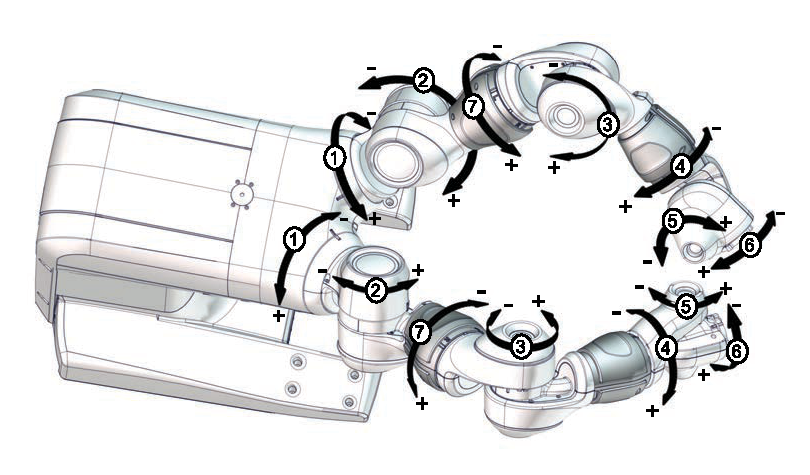
\includegraphics[width=0.7\textwidth]{yumi_konfiguracija.eps}
	\caption{Konfiguracija robota IRB 14000-0.5/0.5}
	\label{fig:yumi_conf}
\end{figure}


\begin{center}
	\begin{tabular}{|lr|c|}
		\hline   Tip &  & ABB IRB 14000-0.5/0.5 \\
		\hline Doseg posamezne roke & & 0.5 $m$ \\
		\hline Nosilnost posamezne roke & & 500 $g$ \\
		\hline Maksimalna hitrost vrha & & 1.5 $m/s$ \\
		\hline Ponovljivost pozicioniranja& & $\pm 0.02 $ $mm$ \\
		\hline Maksimalna hitrost
		& Os 1 & $180$ $^\circ/s$ \\
		& Os 2 & $180$ $^\circ/s$ \\
		& Os 3 & $180$ $^\circ/s$ \\
		& Os 4 & $400$ $^\circ/s$ \\
		& Os 5 & $400$ $^\circ/s$ \\
		& Os 6 & $400$ $^\circ/s$ \\
		& Os 7 & $180$ $^\circ/s$ \\
		\hline Delovni prostor
		& Os 1 & $-168.5^\circ/+168.5^\circ$\\
		& Os 2 & $-143.5^\circ/+43.5^\circ$\\
		& Os 3 & $-123.5^\circ/+80^\circ$\\
		& Os 4 & $-290^\circ/+290^\circ$\\
		& Os 5 & $-88^\circ/+138^\circ$\\
		& Os 6 & $-229^\circ/+229^\circ$\\
		& Os 7 & $-168.5^\circ/+168.5^\circ$\\
		\hline   Teža &  & $38$ $kg$ \\
		\hline   Zavore &  & 1, 2, 3 in 7 os \\
		\hline
	\end{tabular}
\end{center}




Posamezna roka je opremljena z integriranim prijemalom. Prijemalo je sestavljeno iz dveh prstov, ki jih poganjajo servo motorji. Dodan je še en pnevmatski sesek, s katerim se lahko preko vakuuma oziroma komprimiranega zraka manipulira z objekti. Prijemalo na levi roki ima dodatno integrirano kamero proizvajalca Cognex. Prijemalo je prikazano na sliki \ref{fig:yumi_smartgripper}.

\begin{figure}[!hbt]
	\centering
	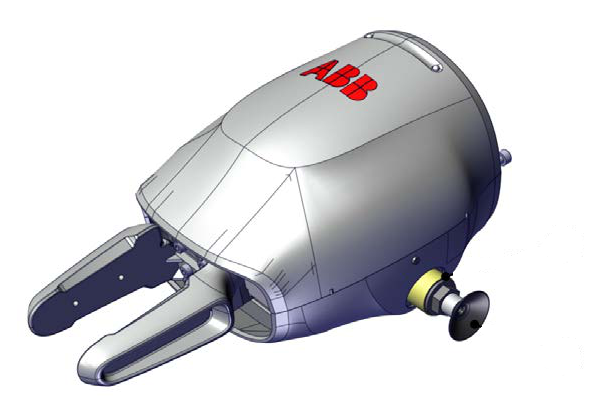
\includegraphics[width=0.5\textwidth]{yumi_smartgripper.eps}
	\caption{Robotsko prijemalo SmartGripper}
	\label{fig:yumi_smartgripper}
\end{figure}


Robota se programira z uporabo ročne učne naprave \emph{FlexPendant} (slika \ref{fig:yumi_flexpendant}). Naprava omogoča premikanje robota, upravljanje s prijemali, pisanje, popravljanje in poganjanje programov ter podobno. Ker je IRB 14000 deklariran kot sodelujoči robot za premikanje ni potrebno držati varnostne tipke na spodnji strani ročne učne naprave kot je to v navadi pri premikanju ostalih robotov proizvajalca ABB. Več o uporabi ročne učne naprave FlexPendat je razloženo v poglavju  \label{Pog:ABB}.


\begin{figure}[!hbt]
	\centering
	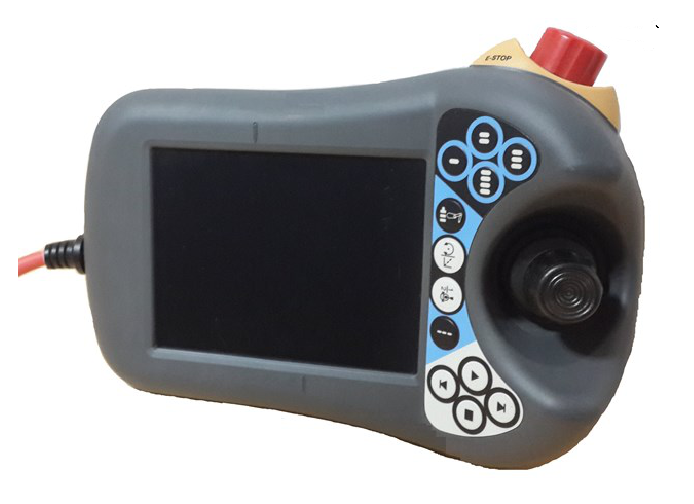
\includegraphics[width=0.5\textwidth]{yumi_flexpendant.eps}
	\caption{Ročna učna naprava \emph{FlexPendant}}
	\label{fig:yumi_flexpendant}
\end{figure}


\section{Dvoročna manipulacija}


\subsection{Ročno vodenje robota}

Ročno vodenje je način vodenja robota s pomočjo krmilne palice. Robota lahko ročno vodite glede na položaje sklepov ali glede na različne koordinatne sisteme. Izbrano delovanje gibanja in/ali koordinatnega sistema določa način premikanja robota. V linearnem načinu gibanja se točka središča orodja (TCP - angl. \emph{tool center point}) premika po ravni črti v prostoru, oz. v smeri osi izbranega koordinatnega sistema. V načinu gibanja ``os-za-osjo'' pa se premika določena os robota. Ker ima krmilna palica tri prostostne stopnje gibanja, lahko naenkrat spreminjate pozicijo le treh koordinat. Ker ime vsaka roka 7 prostostnih stopenj, lahko poleg premikanja vrha premikate tudi sam mehanizem, medtem ko se vrh ne premika.

\begin{figure}[!hbt]
	\centering
	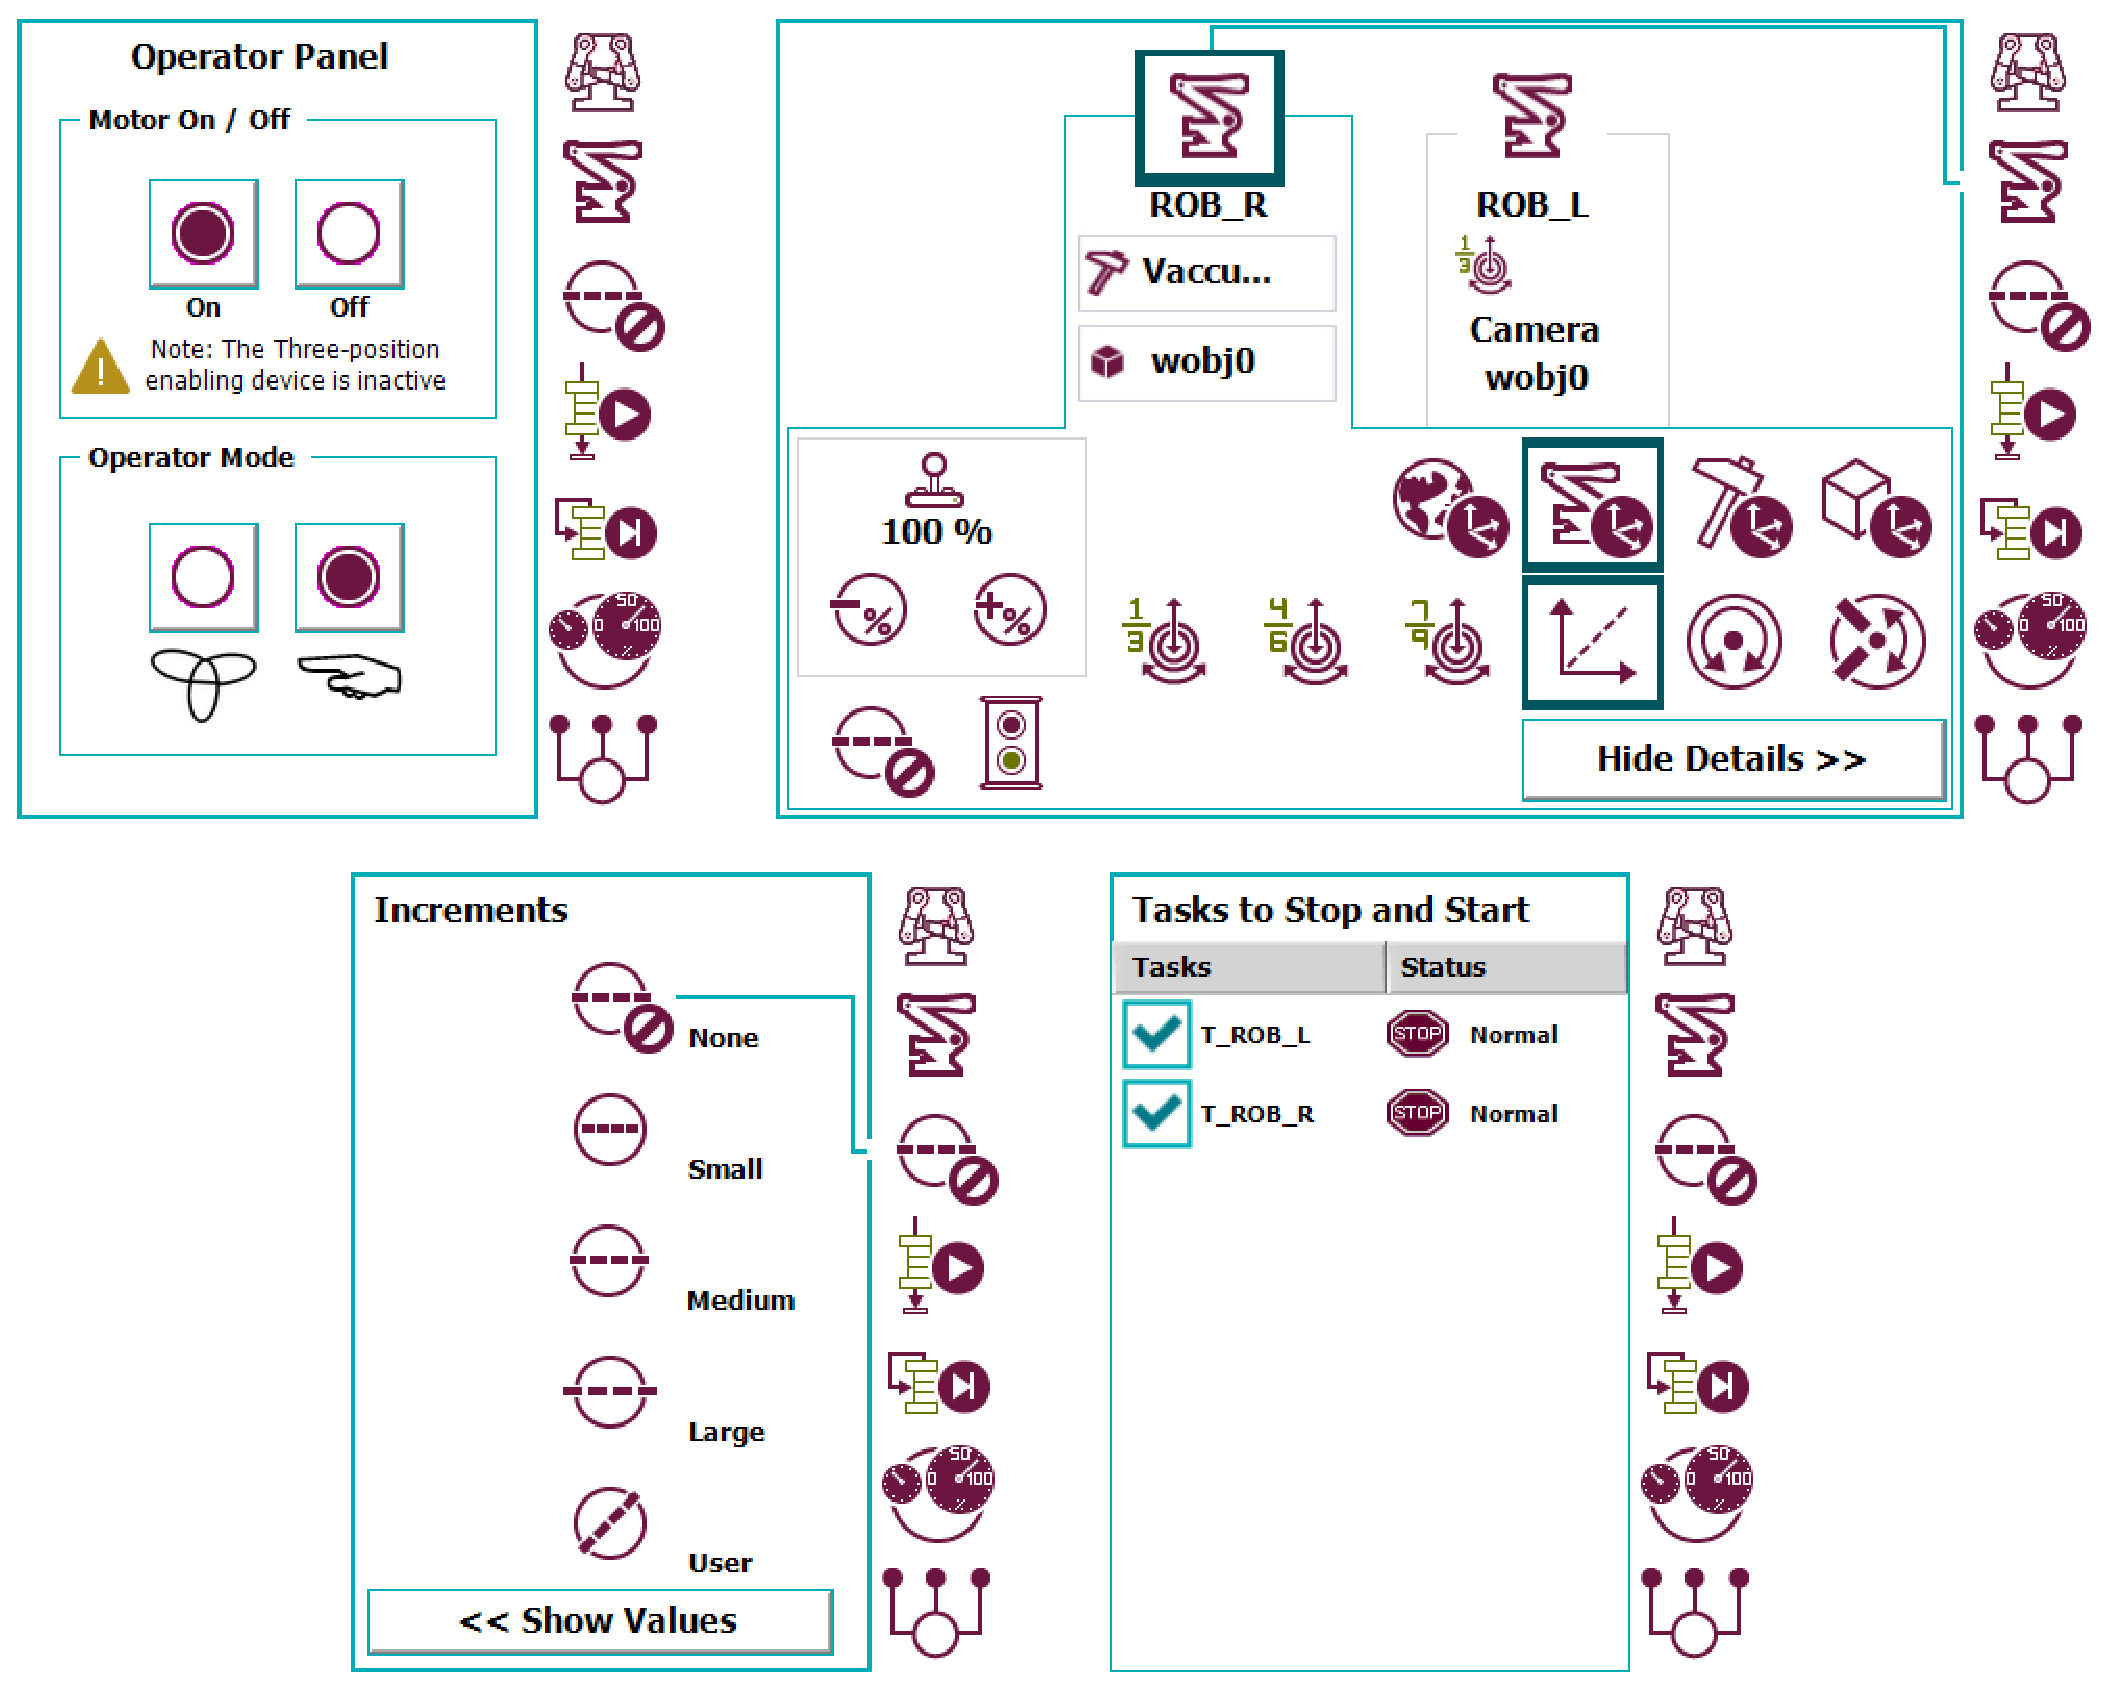
\includegraphics[width=1\textwidth]{yumi_hitri_meni.eps}
	\caption{Hitri meni: Kontrolna plošča (zgoraj levo), izbira načina vodenja (zgoraj desno), inkrementalno vodenje (spodaj levo), izbira aktivnega robota (spodaj desno)}
	\label{fig:yumi_hitri}
\end{figure}

Hitri meni, ki je dostopen preko tipke v spodnjem desnem kotu, nudi osnovno funkcionalnost za premikanje robota. Prvi meni (slika \ref{fig:yumi_hitri} zgoraj levo) je kontrolna plošča, s katero prižigate/ugašate motorje, ter izbirate avtomatski oziroma ročni način izvajanja. Naslednji meni nam podaja izbiro načina vodenja (slika \ref{fig:yumi_hitri} zgoraj desno). Izberete lahko robotsko roko, ki jo želite premikati, izbirate, katere sklepe želite premikati in način premikanja vrha (spreminje pozicije, orientacije ali pa celotne konfiguracije). V tem meniju lahko tudi izberete uporabljeno orodje ter uporabniški koordinatni sistem. Naslednji meni določa hitrost premikanja: pri hitrostnem vodenju je hitrost premikanja proporcionalna odmiku krmilne palice, pri inkrementalnem vodenju pa je premikanje pogojeno z dolžino inkrementa. V naslednjih menijih izbirate način izvajanja programa (program se izvede enkrat ali pa se ponavlja), način premikanja po programu, ter hitrosti, ki omejujejo gibanja robota med učenjem. V zadnjem meniju izberete, kateri robot je aktiven (slika \ref{fig:yumi_hitri} spodaj desno). Na podlagi te izbire morate definirati ustrezne programe; n.p.r. če imate izbrani obe roki, morate ustvariti dva programa, en program za posamezno roko, če pa imate izbrano samo levo roko, pa samo program za levo roko.


\begin{figure}[!hbt]
	\centering
	\includegraphics[width=0.7\textwidth]{yumi_lead.eps}
	\caption{Meni za nastavljanje parametrov vodenja (\emph{Jogging}): izbira robotske roke, načina premikanja, koordinatnih sistemov, orodja, delovnih objektov; meni omogoča tudi izbiro vodenje robota z roko (\emph{Enable Lead-through}).}
	\label{fig:yumi_smart_meni}
\end{figure}

Robot ABB IRB 14000 omogoča tudi vodenje robota z roko (angl. \emph{Lead through}). V tem načinu lahko robotsko roko primemo ter jo postavimo v ustrezno lego; pri tem za premikanje ni potrebno uporabiti krmilne palice. Robotski krmilnik na podlagi modela mehanizma preračunava ustrezne navore za motorje, ki kompenzirajo vpliv vztrajnosti, coriolisovih in centripetalnih sil, statičnega in dinamičnega trenja ter gravitacije. Vsak dodaten navor na motorje, kot je na primer potisk operaterja, predstavlja dodatno komponento navora, ki jo mora robotski mehanizem ustezno izničiti. Ta način vodenja se vklopi z izbiro opcije \TP{\emph{Enable Lead-through}} preko menija \TP{\emph{ABB > Jogging}}. Preden se robotski program požene, je potrebno ta način vodenja izklopiti (\TP{\emph{ABB > Jogging > Disable Lead-through}}).


\subsection{Kreiranje delovnega objekta}

Delovni objekt vsebuje informacijo o novem uporabniškem koordinatnem sistemu. Ta se uporablja za poenostavitev programiranja, ko urejate programe, zaradi prenastavitev določenih opravil, procesov, objektov, itd. Ustvarite jih za poenostavitev premikanja vzdolž površin objektov. Ker jih lahko ustvarite več, je potrebno vedno izbrati tistega, glede na katerega izvajate gibanje. Aktiven koordinatni sistem izberete v meniju \TP{\emph{ABB > Jogging > Workobject}}.

Nov uporabniški koordinatni sistem definirate z \TP{\emph{ABB > Jogging > Workobject > New}}. V novem oknu nastavite ime koordinatnega sistema (\TP{\emph{Name}}), doseg (\TP{\emph{Scope}}) nastavite na globalni, tip shranjevanja (\TP{\emph{Storage Type}}) pa nastavite na \TP{\emph{persistent}}. Ostale nastavitve pustite nespremenjene.

Nov koordinatni sistem je potrebno definirati. To storite z dostopom \TP{\emph{ABB > Jogging > Workobject > Edit > Define}}. Nato izberete želeno metodo kalibracije: \TP{\emph{3 Points}}. Robota ročno vodite v tri določitvene točke, pri čemer prva točka določa izhodišče novega koordinatnega sistema, druga točka smer osi x, pravokotnica na os x, ki teče skozi tretjo točko pa določa os y. Ko robota postavite v ustrezno točko, potrdite pozicijo z \TP{\emph{Modify Position}}. Med samim definiranje ni priporočljivo spremijati orientacije prijemala. Določitev kalibracije zaključite s potrditvijo \TP{\emph{OK}}.


Sintaksa uporabniškega koordinatnega sistema je sledeča:

%{\small
\begin{verbatim}
	wobj:= [FALSE, TRUE, "", [[0,0,0], [1,0,0,0]],
	[[0,0,0], [1,0,0,0]]];
\end{verbatim}
%}

Pri tem prva kombinacija \verb"[[0,0,0], [1,0,0,0]]" predstavlja pozicijo in orientacijo novega koordinatnega sistema glede na bazni koordinatni sistem robota, druga kombinacija \verb"[[0,0,0], [1,0,0,0]]" pa predstavlja lego objekta, definirano v novem koordinatnem sistemu \verb"wobj".

\subsection{Uporaba prijemala}

Robotski roki sta opremljeni z integriranimi robotskimi prijemali. Prijemalo je sestavljeno iz servo motorjev za premikanje prstov, pnevmatike za uporabo vakuuma oziroma izpihavanje ter kamere.

\begin{figure}[!bht]
	\centering
	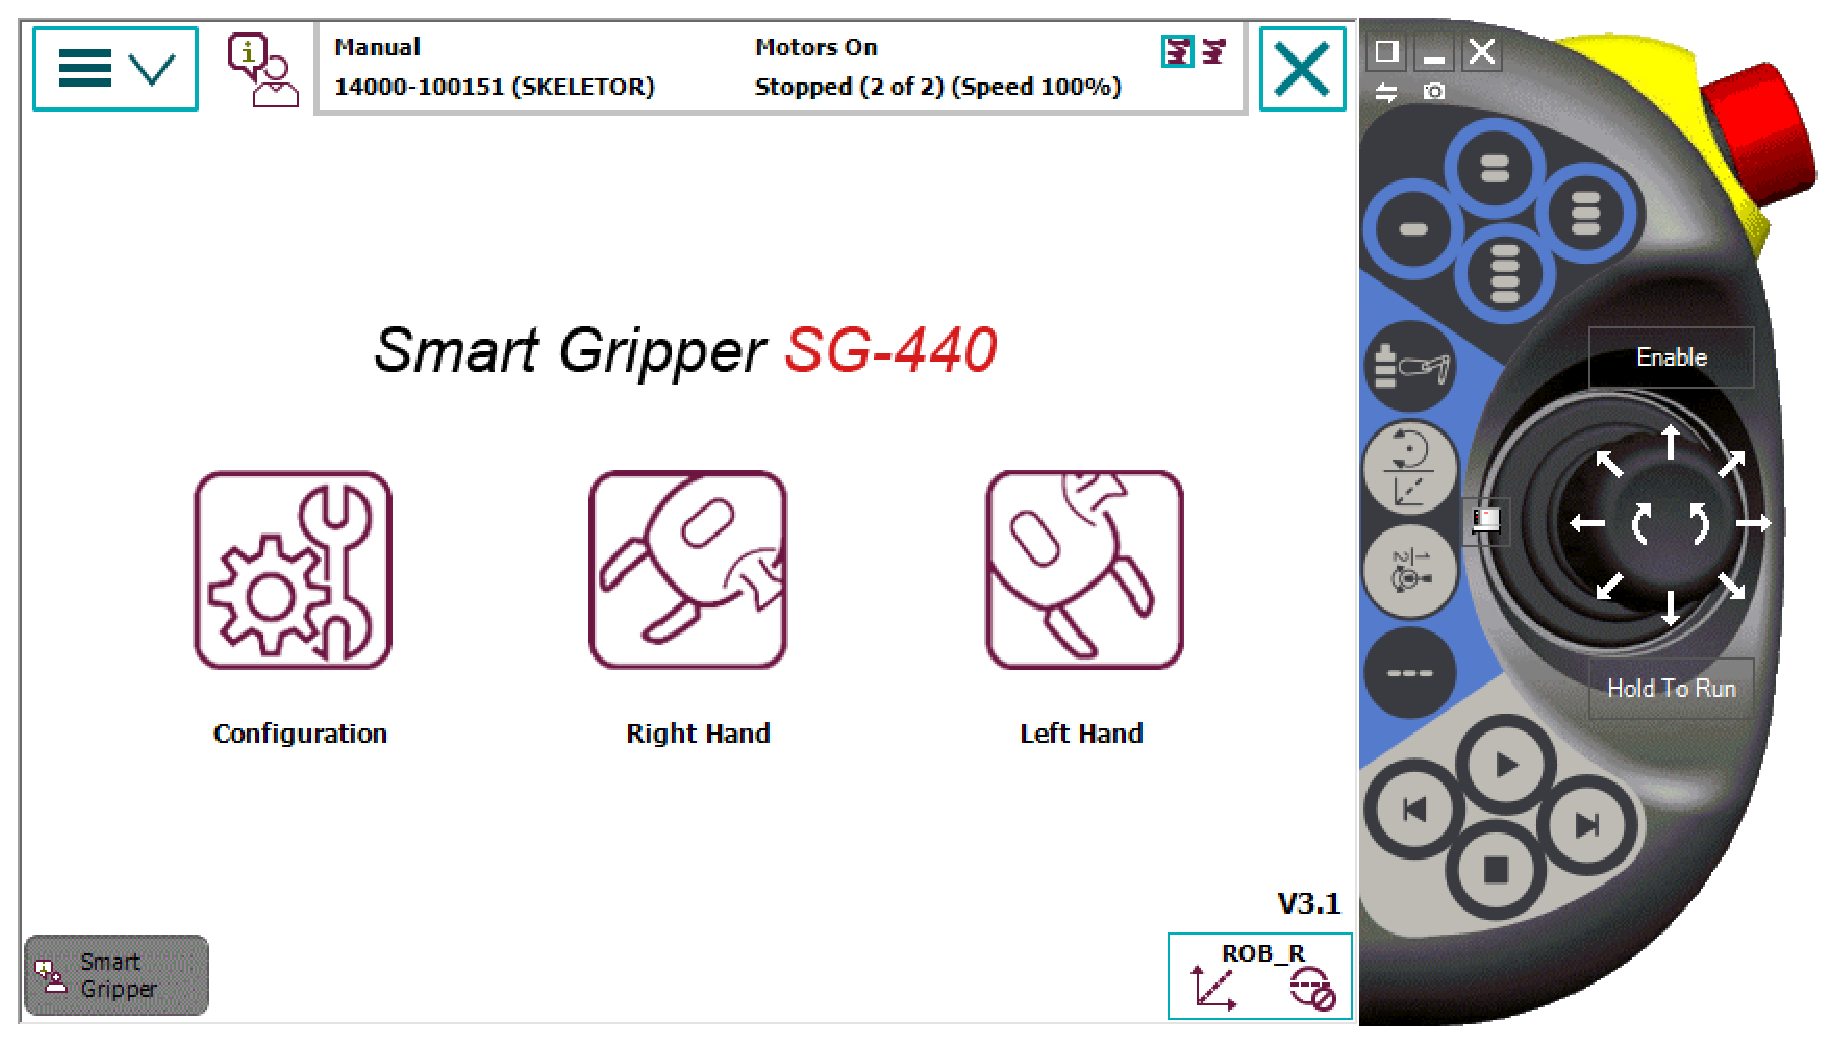
\includegraphics[width=0.7\textwidth]{yumi_smartgripper_meni.eps}
	\caption{Meni za upravljanje z robotskimi prijemali \emph{SmartGripper}}
	\label{fig:yumi_smart_meni}
\end{figure}

Za prijemala obstaja poseben meni, do katerega se dostopa preko \TP{\emph{ABB > Smart Grippers}}. V tem meniju sta na voljo posamezni prijemali ter konfiguracija. Ob kliku na levo ali desno prijemalo se odpre dodatni meni, kjer lahko nastavite hitrost premikanja prstov ter želeno silo prijemanja. Dodatno lahko ročno premikate prijemala (\TP{\emph{Jog$+$}/\emph{Jog$-$}}), premikate prijemalo do željene pozicije (\TP{\emph{Move to}}) oziroma prijemate do nastavljene sile (\TP{\emph{Grip to}}) ter vklapljate/izklapljate vakuum oziroma zrak. Po vsakem zagonu robota je potrebno izvesti kalibracijo prstov, tako da se jih z \TP{\emph{Jog$-$}} stisne ter nato izbere gumb \TP{\emph{Calibrate}}. Indikator ob gumbu sporoča stanje prijemala (zelena - prijemalo je kalibrirano, rdeča - prijemalo je potrebno kalibrirati). V program se lahko vključi sledečo kodo, ki v primeru, da prijemala niso kalibrirana, izvede inicializacijo (nastavi maksimalno hitrost na 20 mm/s ter silo prijemanja na 10 N) ter kalibracijo.



%{\small
\begin{verbatim}
	IF Hand_IsCalibrated() THEN
	!roka je ze kalibrirana
	ELSE
	Hand_Initialize \maxSpd:=20, \holdForce:=10,
	\Calibrate;
	ENDIF
\end{verbatim}
%}

Prijemalo se krmili z ukazi, ki so v programu na voljo preko \TP{\emph{Add instruction}}, kjer izberete \TP{\emph{SmartGripper}}. Za premikanje prstov so na voljo sledeči ukazi:
\begin{itemize}
	\item \verb"Hand_JogInward" se uporablja za premikanja prijemala navznoter; prijemalo se ne ustavi, dokler ne doseže mehanske omejitve;
	\item \verb"Hand_JogOutward" se uporablja za premikanja prijemala navzven; prijemalo se ne ustavi, dokler ne doseže mehanske omejitve;
	\item \verb"Hand_MoveTo" premakne prijemalo do nastavljene pozicije;
	\item \verb"Hand_GripInward" se uporablja za premikanje prijemala navznoter; nastavlja se lahko dodatne parametre: sila držanja \verb"\holdForce", željena pozicija \verb"\targetPos";
	\item \verb"Hand_GripOutward" se uporablja za premikanje prijemala navzven; nastavlja se lahko dodatne parametre: sila držanja \verb"\holdForce", željena pozicija \verb"\targetPos".
\end{itemize}
Za manipulacijo pnevmatike se uporabljajo sledeči ukazi:
\begin{itemize}
	\item \verb"Hand_TurnOnBlow1" vklopi pihanje na kanalu 1;
	\item \verb"Hand_TurnOffBlow1" izklopi pihanje na kanalu 1;
	\item \verb"Hand_TurnOnVacuum1" vklopi vakuum na kanalu 1;
	\item \verb"Hand_TurnOffVacuum1" izklopi vakuum na kanalu 1.
\end{itemize}
Podobni ukazi veljajo tudi za drugi kanal. V programu RobotStudio so ukazi na voljo v zavihku \TP{\emph{RAPID > Instruction > SmartGripper}}.

\subsection{Program RAPID}

Robotski program je sestavljen iz niza ukazov, ki opisujejo kam in na kakšen način naj se robot premakne. Ker je robot IRB 14000 sestavljen iz dveh robotskih rok sta potrebna dva ločena programa. Dostop do programov je preko \TP{\emph{ABB > Program Editor}}. Tu lahko izberete program za levo (\verb"T_ROB_L") ali desno roko (\verb"T_ROB_R").

\begin{figure}[!hbt]
	\centering
	\includegraphics[width=0.7\textwidth]{yumi_program_editor.eps}
	\caption{Pregled programov, ki so naloženi za posamezno robotsko roko}
	\label{fig:yumi_program_editor}
\end{figure}

Nov program ustvarite z izbiro \TP{\emph{File > New Program}}, že napisan program pa naložite z \TP{\emph{File > Load Program}}. Program shranite z \TP{\emph{File > Save Program As}}.

%\begin{figure}[!hbt]
%\centering
%\includegraphics[width=0.7\textwidth]{yumi_program.eps}
%\caption{Primer kratkega programa za levo roko}
%\label{fig:yumi_program_L}
%\end{figure}

Za učenje programa morate robota najprej postaviti v željeno lego. Nato željeno lego shranite z izbiro \TP{\emph{Add Instruction}}, v dodatnem meniju pa izberete ukaz, ki definira način premika robota v to točko. Največkrat uporabljeni ukazi so
\begin{enumerate}
	\item \verb"MoveJ" - koordinirano gibanje po sklepih;
	\item \verb"MoveL" - linearno gibanje vrha robota;
	\item \verb"MoveC" - krožno gibanje vrha robota.
\end{enumerate}

\begin{figure}[!tbh]
	\centering
	\includegraphics[width=0.7\textwidth]{yumi_program.eps}
	\caption{Primer kratkega programa za levo roko}
	\label{fig:yumi_program_L}
\end{figure}

Sintaksa posameznega ukaza je sledeča:
{\small
	\begin{verbatim}
		[MotionType] [Name], [Speed], [Zone], [Tool], [WorkObject];
	\end{verbatim}
}
Posamezne komponente so
\begin{enumerate}
	\item \verb"[MotionType]" definira način premikanja robota;
	\item \verb"[Name]" je ime točke, ki definira lego robota; če ime ni definirano, je nadomeščeno z zvezdico \verb"*";
	\item \verb"[Speed]" definira hitrost robota;
	\item \verb"[Zone]" definira, kako natančno naj robot pride/obide točko; \verb"fine" določa, da robot pride točno v točko in se tam ustavi;
	\item \verb"[Tool]" definira TCP, katerega naj robot postavi v izbrano točko;
	\item \verb"[WorkObject]" definira koordinatni sistem, glede na katerega je definirana točka.
\end{enumerate}

\section{Robotski vid}

Robot ABB IRB 14000-0.5/0.5 ima v levem prijemalu integrirano industrijsko kamero Cognex In-Sight serije 7000. V industriji se robotski vid uporablja za iskanje in pregled objektov, merjenje objektov ter preverjanje posameznih značilk.

Kamera, nameščena v prijemalu robota, lahko zajema slike s hitrostjo do 102 sliki na sekundo z resolucijo $800 \times 600$ slikovnih pik. Dodatno ima integrirano osvetlitev z LED diodo. Kameri je mogoče nastaviti čas odprtja zaslonke, način in interval proženja, intenziteto osvetlitve, ipd. Do nastavitev kamere dostopate preko programskega okolja EasyBuilder, ki je integriran v programski paket RobotStudio.

\begin{figure}[!hbt]
	\centering
	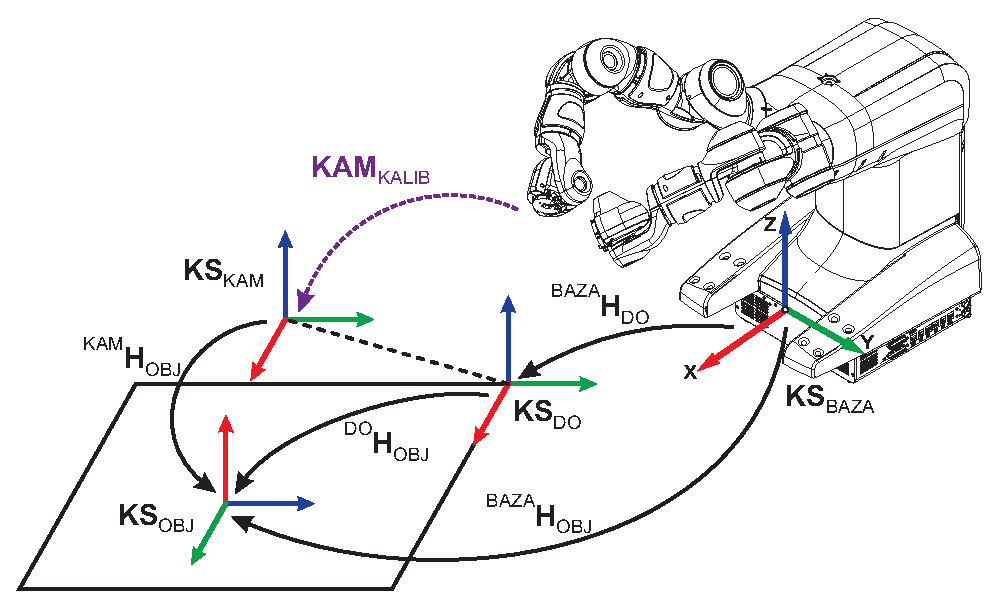
\includegraphics[width=0.8\textwidth]{yumi_cam_wobj.eps}
	\caption{Postavitev koordinatnih sistemov. Koordinatni sistem kamere $\textbf{KS}_{KAM}$ in koordinatni sistem delovnega objekta $\textbf{KS}_{DO}$ sta soležna, kar nakazuje črtkana črta.}
	\label{fig:yumi_kam_wobj}
\end{figure}


Predno lahko uporabite kamero, je le-to potrebno kalibrirati s pomočjo različnih kalibracijskih mrež. S kalibracijo se določi transformacijo med slikovnimi točkami in milimetri, obenem pa se določi tudi koordinatni sistem kamere, ki je pripet na samo kalibracijsko mrežo. Da se podatke iz kamere lahko uporabi za robota, je potrebno definirati še uporabniški koordinatni sistem, ki soupada s koordnitanim sistemom kamere. Tako je lega prepoznanega objekta v koordinatnem sistemu kamere enaka legi objekta v uporabniškem koordinatnem sistemu. Relacije med koordinatnimi sistemi so prikazane na sliki \ref{fig:yumi_kam_wobj}.

%\vspace{5mm}

\newpage
\begin{mdframed}[backgroundcolor=blue!20, shadow=true,roundcorner=8pt]
	\textbf{Primer:}Program za prepoznavo objekta s kamero najde objekt na poziciji ${}^{KAM}\textbf{KS}_{OBJ} = [0.3\, 0.15\, 0]$ glede na izhodišče kamere $\textbf{KS}_{KAM}$. Ker je uporabniški sistem $\textbf{KS}_{DO}$ poravnan s koordinatnih sistemom kamere $\textbf{KS}_{KAM}$ velja, da je objekt na poziciji ${}^{DO}\textbf{KS}_{OBJ} = [0.3\, 0.15\, 0]$ glede na izhodišče delovnega objekta $\textbf{KS}_{DO}$. Ker je delovni objekt definiran glede na bazni koordinatni sistem robota, je lega objekta določena
	\begin{equation*}
		{}^{BAZA}\textbf{H}_{OBJ} = {}^{BAZA}\textbf{H}_{DO}  {}^{DO}\textbf{H}_{OBJ} \,.
	\end{equation*}
\end{mdframed}


\section{Prepoznava in manipulacija objektov}

Vaja je sestavljena iz več sklopov:
\begin{itemize}
	\item priprava programa RAPID;
	\item kalibracija kamere ter povezava robota in kamere;
	\item priprava programa robotskega vida za prepoznavo objekta;
	\item definiranje prijemanja objekta;
	\item definiranje točk odlagajanja objekta;
	\item nadgradnja programa za prepoznavo in manipulacijo treh objektov.
\end{itemize}

\subsection{Priprava programa}

Pri tej vaji boste uporabljali samo levo robotsko roko, ker je na njej nameščena kamera. Preko hitrega menija nastavite kot aktivno roko samo levo roko, ter za njo ustvarite nov program (\TP{\emph{ABB > Program editor > Task and programs > File > New program}}). Program shranite v mapo \verb"HOME\Programi\OSNOVE_ROBOTIKE".

Nato se povežete na krmilnik robota s programsko opremo RobotStudio. To storite tako, da poženete program RobotStudio in v zavihku \RS{\emph{Controller}} kliknete \RS{\emph{Add Controller}}. Nato izberete še opcijo \RS{\emph{Request Write Access}}, na ročni učni napravi pa izberete \TP{\emph{Grant}}. S tem dovolite, da uporabnik RobotStudia pridobi pravice za spreminjanje programa.

Na levi strani v zavihku \RS{\emph{Controller > RAPID}} odprite drevesno strukturo za levo roko (\RS{\emph{T\_ROB\_L}}); pri tem se vam odpre seznam uporabljenih modulov. Izberite \RS{\emph{MainModule}}. Vrstici \verb"PROC Main()" in \verb"ENDPROC" nadomestite s predpripravljeno kodo - t.i. \emph{Snippets}. Do te kode dostopate preko zavihka \RS{\emph{RAPID}}, kjer izberete \RS{\emph{Snippet > OR\_vaje\_2}}.

\begin{figure}[!hbt]
	\centering
	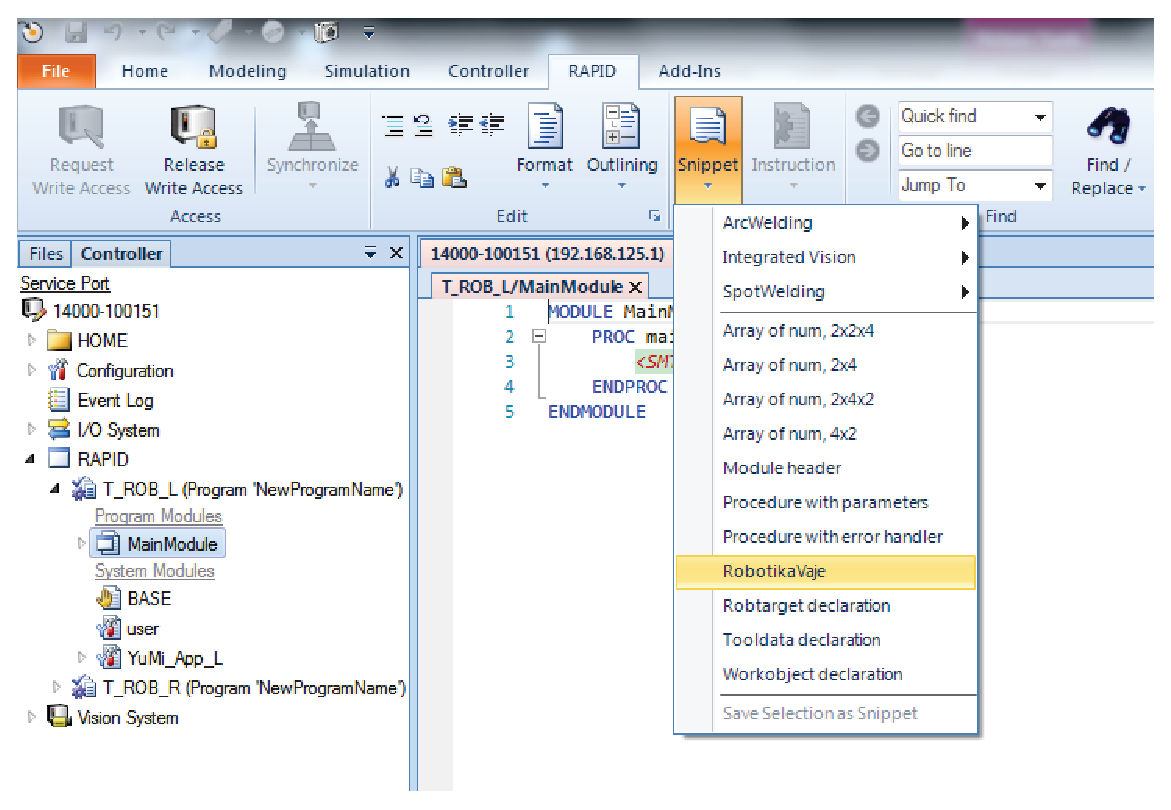
\includegraphics[width=0.9\textwidth]{yumi_snippet2.eps}
	\caption{Drevesna struktura naloženih programov na krmilniku ter \emph{Snippet} meni}
	\label{fig:yumi_snippet}
\end{figure}

Program boste ustrezno spreminjali med nadaljevanjem vaje. Program boste spreminjali tam, kjer je označeno z značko
%{\small
\begin{verbatim}
	!##### STUDENT #####
	...
	!###################
\end{verbatim}
%}

Program naložite na krmilnik tako, da kliknete na gumb \RS{\emph{Apply}} v zavihku \RS{\emph{RAPID}}.

\vspace{5mm}

\begin{mdframed}[backgroundcolor=yellow!20, shadow=true,roundcorner=8pt]
	\textbf{Koraki za izvedbo naloge:}
	\begin{itemize}
		\item za aktivno roko izberite samo levo roko: \TP{\emph{hitri meni > Tasks to Stop and Start}};
		\item ustvarite nov program za levo roko: \TP{\emph{ABB > Program editor > Task and programs > File > New program}};
		\item povežite RobotStudio in krmilnik robota: \RS{\emph{Controller > Add Controller}};
		\item zahtevajte dovoljenje za pisanje v RobotStudiu: \RS{\emph{Request Write Access}};
		\item namesto \verb"PROC Main ... ENDPROC" vstavite predpripravljeno kodo za prijemanje objektov: \RS{\emph{Snippet > RobotikaVaje}};
		\item program naložite na krmilnik \RS{\emph{RAPID > Apply}}.
	\end{itemize}
\end{mdframed}


\subsection{Kalibracija kamere}
\label{ch:kalibracija_kamere}

Ko se povežete na robotski krmilnik, se vam pri drevesni strukturi pojavi možnost \RS{\emph{Vision System}}. če kliknete na puščico poleg imena, se vam pokaže aktivna kamera - v našem primeru je to kamera z imenom \RS{\emph{Yumi\_Vision}}. Zavihek \RS{\emph{Vision}} se vam odpre, če kliknete DMK na \RS{\emph{Vision System}} in izberete \RS{\emph{Integrated Vision}}. S kamero se povežete, če kliknete na gumb \RS{\emph{Connect}}, ki se nahaja na levi strani v zavihku \RS{\emph{Vision}}. Ko je kamera povezana, lahko naredite posnetek s klikom na \RS{\emph{Acquire Image}}. Nastavitve kamere vam omogočajo, da nastavite optimalno sliko. Najpomembnejši nastavitvi sta čas odprtja zaslonke (angl. \emph{Exposure}) in intenziteta osvetlitve (angl. \emph{Light Intensity}). Do nastavitev dostopa preko gumba \RS{\emph{Setup Image}}. Priporočljivo je zmanjšati osvetlitev, ali pa jo kar izklopiti (\emph{Light Control Mode} nastavite na \emph{Disabled}).

Najprej ustvarite nov program za uporabo kamere (angl. \RS{\emph{Vision Job}}). To storite z \RS{\emph{New Job}} v zavihku \emph{Vision}. Kliknite \RS{\emph{Yes}} ter program shranite na samo kamero ter ga poimenujte (klik na \RS{\emph{Save Job}}). Ta program boste med izvedbo vaje naložili v delovni pomnilnik kamere. V RAPID kodi zamenjajte ime programa \verb"mojrobotskivid.job" z imenom vašega programa.

Pred uporabo je potrebno kamero kalibrirati, kjer se določi pretvorbo med slikovnimi pikami in milimetri ter korekcijo zaradi ukrivljenosti leče oziroma projekcije. Pri tem boste uporabili natisnjeno šahovnico, ki jo postavite na mizo. Levo robotsko roko z uporabo ročne učne naprave postavite v tako lego, da vidite celotno šahovnico. Ko ste zadovoljni s postavitvijo, to shranite v vašem RAPID programu. To storite tako, da na ročni učni enoti izberete vrstico
%{\small
\begin{verbatim}
	MoveJ polozajKamere, v300, fine, GripperL;
\end{verbatim}
%}
ter kliknete \TP{\emph{Modify Position}}. Ta točka vam predstavlja lego kamere, v kateri boste morali postavi robota pred uporabo kamere.

\begin{figure}[!tb]
	\centering
	\includegraphics[width=0.9\textwidth]{yumi_kam_kalibracija.eps}
	\caption{Primer kalibracije kamere}
	\label{fig:yumi_kam_kalib}
\end{figure}


Kalibracijo se izbere s klikom na gumb \RS{\emph{Calibrate}} v RobotStudiu. Odpre se vam okno, kjer izberete tip kalibracije. Izberete \RS{\emph{Grid}} ter preverite, če je razdalja med kockami nastavljena na 10~mm. Nato kliknete \RS{\emph{Next}}. V naslednjem koraku program za kalibracijo prepozna posamezna polja, ki se vam izpišejo na zaslonu. če so polja lepo vidna, nadaljujete s kalibracijo. V nasprotnem primeru ustrezno popravite postavite robota/mreže oziroma parametre slike. Kalibracijo poženete s klikom na gumb \RS{\emph{Calibrate}}. Grafični prikaz vam pokaže kvaliteto kalibracije. če je rezultat zadovoljiv,  zaključite z izbiro \RS{\emph{Finish}}. Program shranite z gumbom \RS{\emph{Save Job}}.


\vspace{5mm}

\begin{mdframed}[backgroundcolor=yellow!20, shadow=true,roundcorner=8pt]
	\textbf{Koraki za izvedbo naloge:}
	\begin{itemize}
		\item odprite zavihek \RS{\emph{Vision}: \emph{Controller > Integrated Vision}};
		\item povežite se s kamero: \RS{\emph{Controller > Connect}};
		\item kreirajte nov program robotskega vida: \RS{\emph{Vision > New Job}};
		\item program robotskega vida poimenujte in shranite: \RS{\emph{Vision > Save Job}};
		\item v predpripravljeni kodi nadomestite \verb"mojrobotskivid.job" z imenom vašega programa;
		\item levo robotsko roko postavite tako, da vidite celotno šahovnico; sliko pogledate z \RS{\emph{Vision > Acquire Image}};
		\item shranite točko v robotski program: v programu se postavite na točko \verb"polozajKamere" ter izberete \TP{\emph{Modify Position}};
		\item naredite kalibracijo: \RS{\emph{Vision > Calibrate}}.
	\end{itemize}
\end{mdframed}


\subsection{Povezava kamere in robota}


Po kalibraciji kamere so vse izhodne vrednosti programov za obdelavo slike podane v koordinatnem sistemu kamere. Da lahko robot pravilno interpretira podatke s kamere, ga je potrebno naučiti lego koordinatnega sistema kalibrirane kamere. S tem se definira skupen koordinatni sistem, ki povezuje kamero in robota.

To storite tako, da definirate delovni objekt, ki vsebuje informacije o uporabniškem koordinatnem sistemu ter koordinatnem sistemu objekta. S to kalibracijo spremenite samo uporabniški koordinatni sistem, koordinatni sistem objekta pa ostane nespremenjen. Uporabniški koordinatni sistem je določen s postavitvijo kalibracijske mreže, ki mora biti postavljena enako kot pri kalibraciji kamere. V prijemalo leve roke vpnete orodje s špico, ki jo boste uporabili za definiranje novega koordinatnega sistema (\TP{\emph{ABB > Smart Grippers > Left Hand > Grip to [0] mm}}). Kot orodje leve roke izberete \verb"CalibSpikeL" (\TP{\emph{ABB > Jogging > Tool > CalibSpikeL}}). Delovni objekt definirate tako, da preko menija \TP{\emph{ABB}} izberete \TP{\emph{Jogging}}, nato pa s klikom na polje poleg \TP{\emph{Work object:}} odprete seznam uporabniških koordinatnih sistemov. Izbere koordinatni sistem \verb"wobjKamere". Nato z \TP{\emph{Edit > Define}} začnete z definicijo koordinatnega sistema, pri čemer izberete metodo s 3 točkami (\TP{\emph{User method: 3 points}}). Prva točka je postavljena na presečišču premic, ki opisujeta krajši stranici pravokotnikov na šahovnici, druga točka je nekje na osi v smeri osi x, tretja pa na osi y. Te točke so prikazane na sliki \ref{fig:yumi_grid}. Določitev kalibracije zaključite s potrditvijo \TP{\emph{OK}}.


\begin{figure}[!t]
	\centering
	\includegraphics[width=0.95\textwidth]{yumi_grid.eps}
	\caption{Mreža za kalibracijo kamere z označenim izhodiščem}
	\label{fig:yumi_grid}
\end{figure}

Po končani kalibraciji še preverite, ali je delovni objekt ustrezno definiran. V hitrem meniju nastavite za delovno objekt \verb"wobjKamere" (druga ikona pod izbranim robotom), izberete vodenje glede na delovni objekt (ikona kocke s koordinatnim sistemom) ter premikakanje po oseh (ikona grafa s črtkano črto). če sedaj robota premikate s krmilno palico po posameznih oseh, bi se moral vrh robota premikati vzporedno glede na kalibracijsko mrežo.

\vspace{5mm}
\begin{mdframed}[backgroundcolor=yellow!20, shadow=true,roundcorner=8pt]
	\textbf{Koraki za izvedbo naloge:}
	\begin{itemize}
		\item v levo robotsko roko vpnite kalibracijsko konico: \TP{\emph{ABB > Smart Grippers > Left Hand > Grip to: [0] mm}}
		\item nastavite orodje \verb"CalibSpikeL": \TP{\emph{ABB > Jogging > Tool}};
		\item izberete delovni objekt \verb"wobjKamere": \TP{\emph{ABB > Jogging > Work object}};
		\item definirajte točke delovnega objekta: \TP{\emph{Edit > Define}}; izberete \TP{\emph{User method: 3 points}};
		\item robotsko roko postavite v središče koordinatnega sistema, ter točko \verb"User Point X 1" shranite z \TP{\emph{Modify Position}}; enako naredite še za točki na osi x (\verb"User Point X 2") in osi y (\verb"User Point Y 1");
		\item potrdite definicijo novega delovnega objekta z \TP{\emph{OK > OK > OK}};
		\item preiskusite premikanje robota glede na delovni objekt \verb"wobjKamere".
	\end{itemize}
\end{mdframed}

\subsection{Definiranje naloge robotskega vida}
\label{ch:vision_job}

Ko zaključite s kalibracijo kamere lahko odstranite mrežo, v vidni prostor kamere pa postavite objekt, ki ga želite prepoznati. Robota postavite v položaj za slikanje: \TP{\emph{Jogging > Go To...}}, izberete \verb"polozajKamere" ter pritisnete in držite \TP{\emph{Go to}} dokler se robot ne postavi v pravilno lego. Pri tem pazite, da imate izbran delovni objekt \verb"wobj0". Zatem preverite kvaliteto slike (\RS{\emph{Vision > Acquire Image}}); če je potrebno, ustrezno nastavite parametre kamere preko menija \RS{\emph{Setup Image}}.

Za prepoznavo objektov sta na voljo dva tipa orodij: orodja za določitev lege (\RS{\emph{Part Location Tool}}) in orodja za preverjanje objektov (\RS{\emph{Part Inspection Tool}}). Pri tej vaji vas bo zanima lega objektov, zato boste uporabili orodja za določitev lege. Dostopna so preko zavihka \RS{\emph{Vision > Add Part Location Tool}}. Med bolj pogosto uporabljenimi orodji sta {\emph{PatMax}} in {\emph{Blob}} ter njuni različici {\emph{PatMax(1-10)}} in {\emph{Blob(1-10)}}, ki omogočata prepoznavo do 10 enakih objektov. Orodje {\emph{PatMax}} nam omogoča prepoznavo objektov na podlagi geometrijskih značilk. Orodje {\emph{Blob}} pa spremlja, kje se nahajajo različne intenzitete barve, ki predstavljajo opazovane objekte.

\begin{figure}[!hbt]
	\centering
	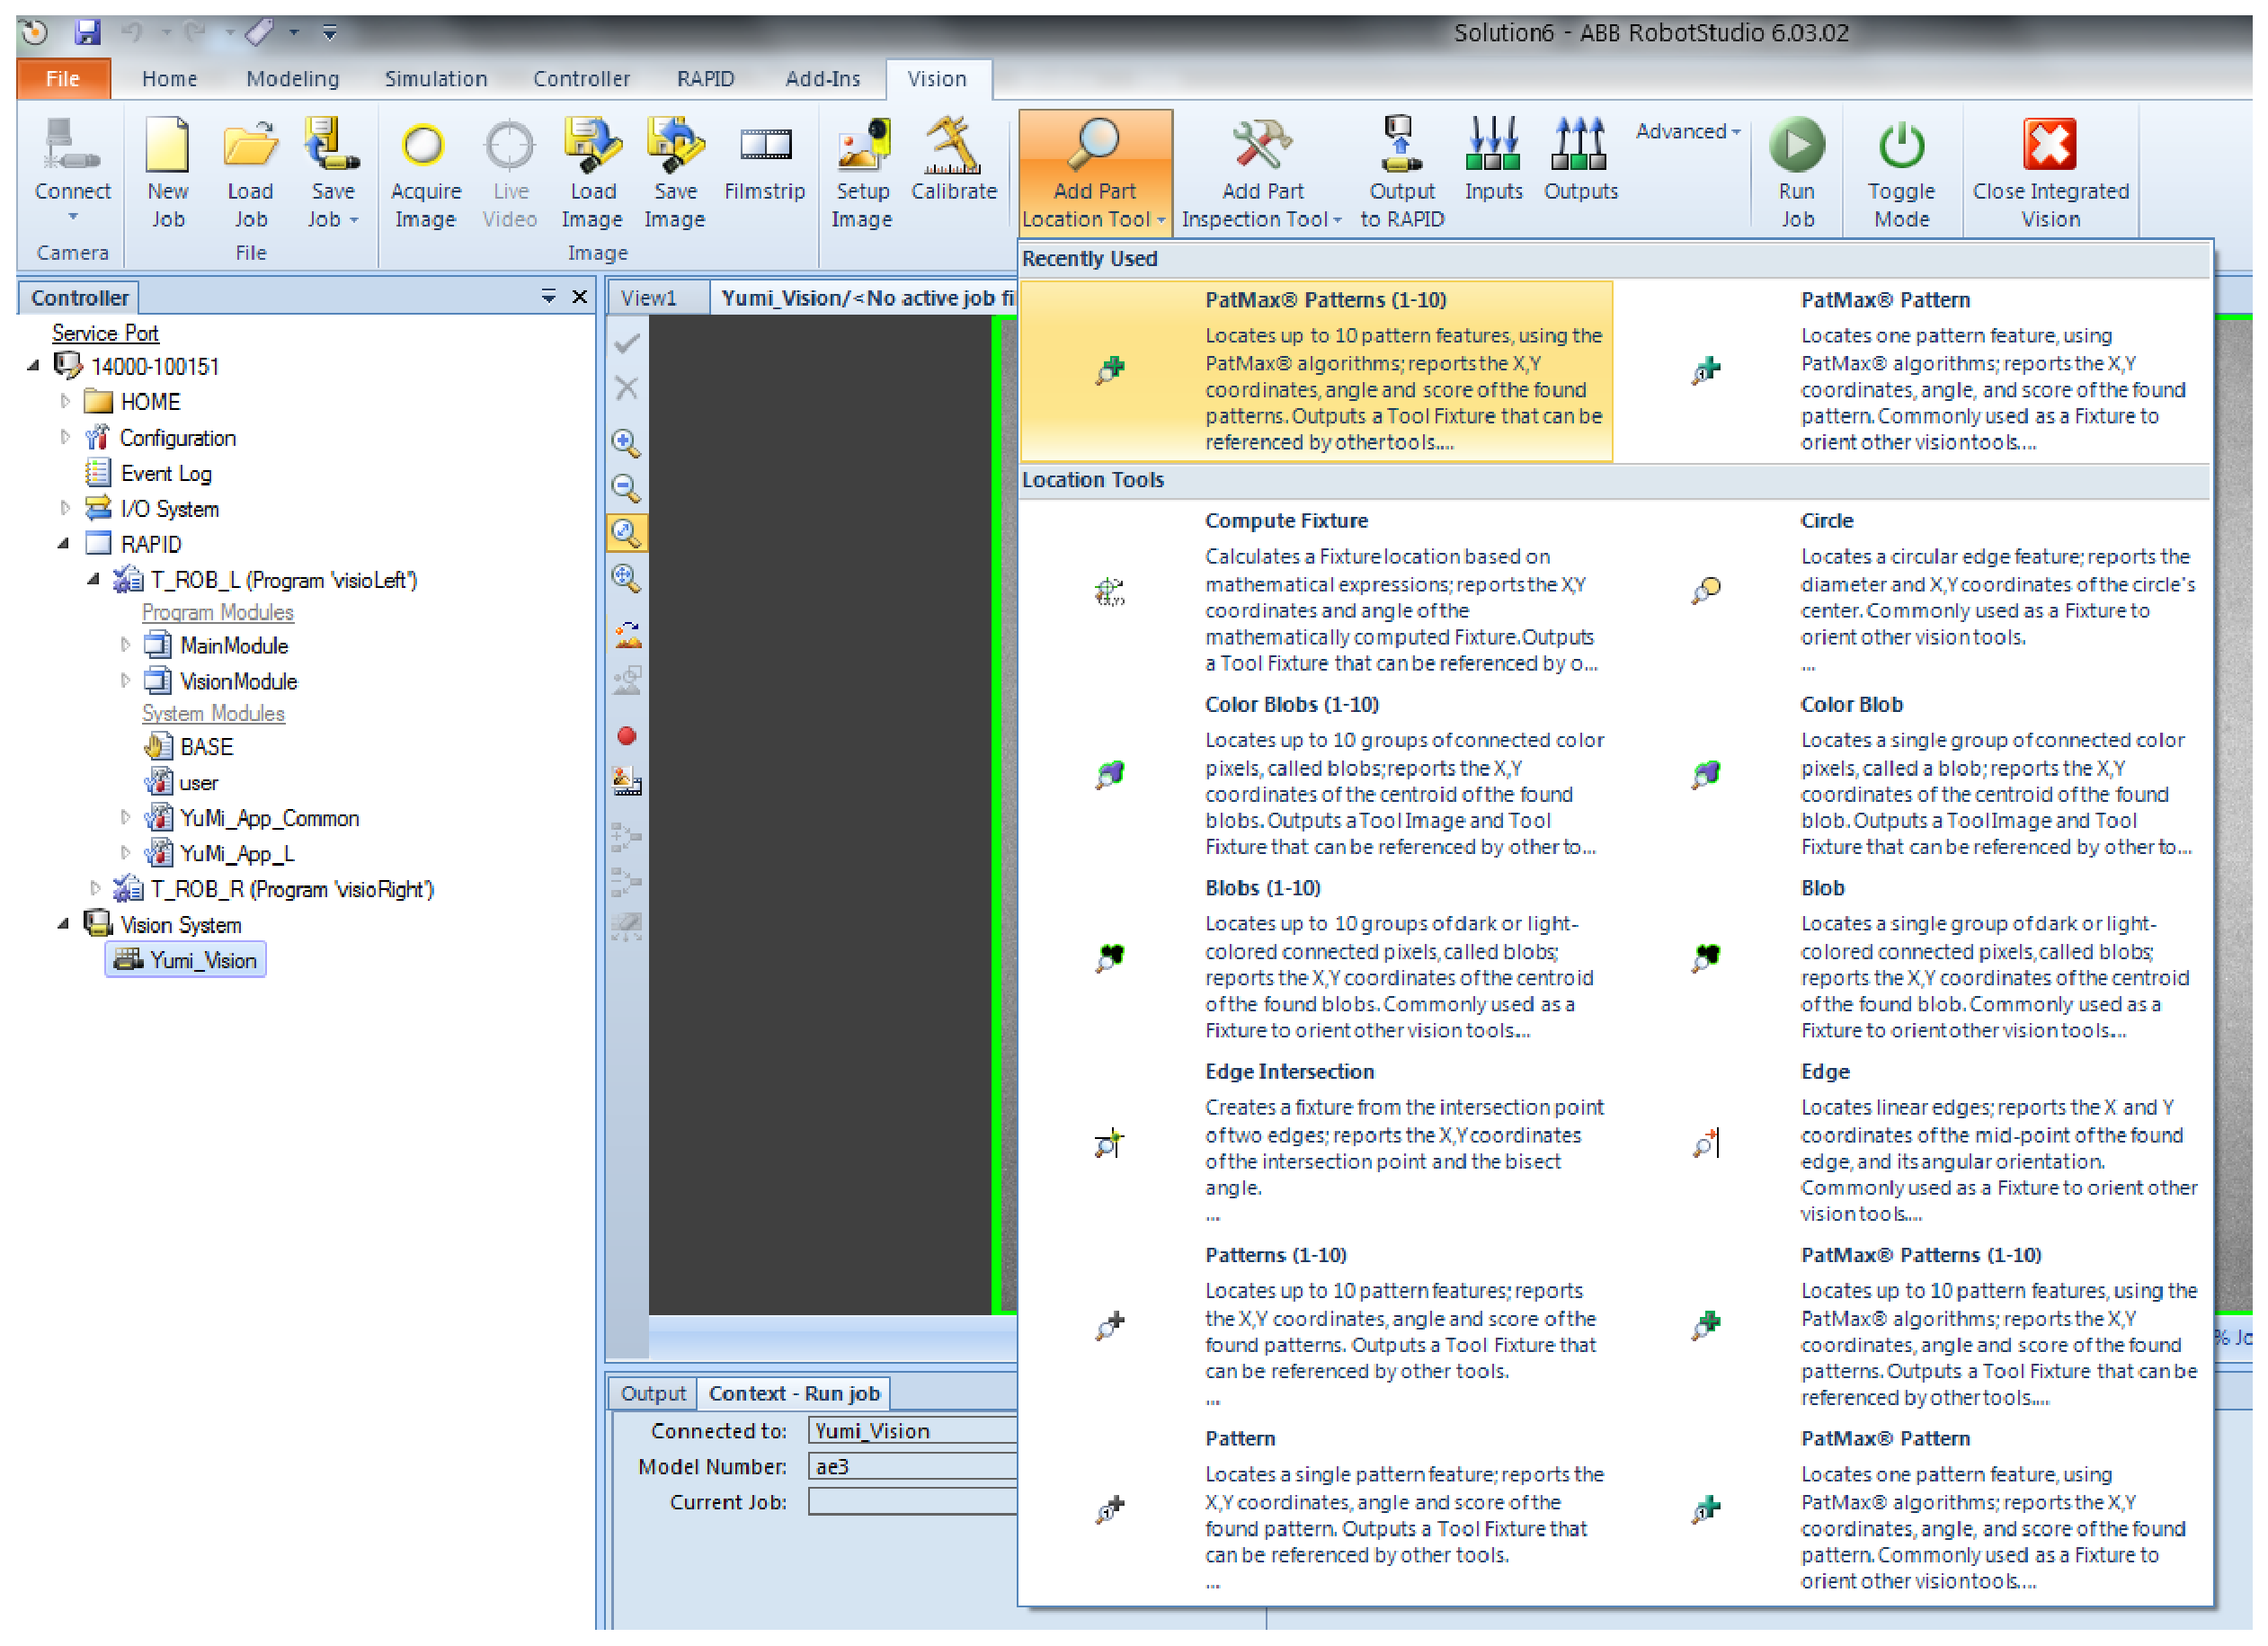
\includegraphics[width=0.9\textwidth]{yumi_location_tool.eps}
	\caption{Meni z različnimi orodji za prepoznavo objektov}
	\label{fig:yumi_location_tool}
\end{figure}

Pri tej nalogi boste uporabili orodje {\emph{PatMax}}. To orodje se uporablja za določitev pozicije posameznih značilk objekta. Temelji na vnaprej naučenem modelu objekta. Orodje {\emph{PatMax Pattern Tool}} se uporablja za določitev enega samega objekta, medtem ko se {\emph{PatMax Patterns (1-10)}} uporablja za določitev pozicije do 10 objektov.

Ko izberete orodje \RS{\emph{Pat Max Patterns (1-10)}}, je potrebno definirati področje modela (ang. Model Region) ter področje, kjer se objekt lahko nahaja (ang. Search Region). Področje modela je lahko pravokotnik, krog, obroč ali poligon. Izbrano področje ustrezno prestavite nad model. Pri tem pazite, da izbrano področje pokriva samo pomembne značilke objekta.

Nato je potrebno definirati področje iskanja. To področje je lahko pravokotnik, krog, obroč ali poligon. Izbira naj pokriva področje, kjer se pričakuje, da bo objekt. Velikost področja vpliva na hitrost delovanja algoritma: večje kot je področje, več časa bo porabil algoritem za analizo. Ko nastavite obe ustrezni področji potrdite izbiro z \RS{\emph{OK}}.

\begin{figure}[!hbt]
	\centering
	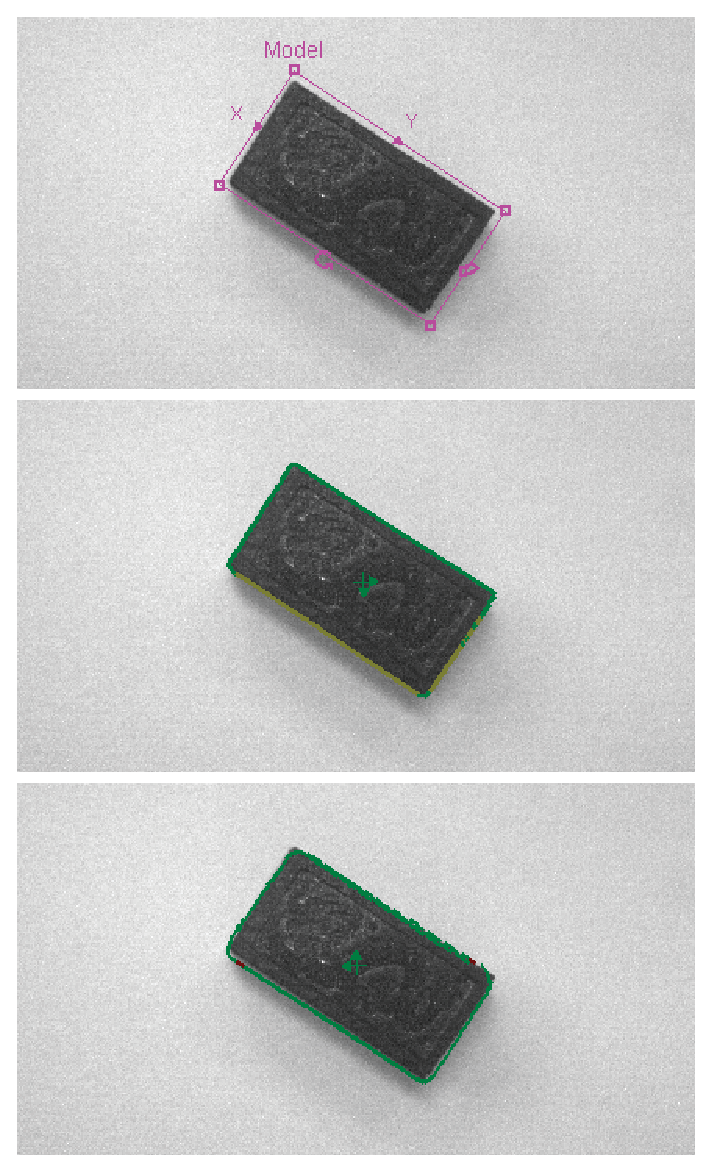
\includegraphics[width=0.6\textwidth]{yumi_vision2.eps}
	\caption{Učenje prepoznave novega objekta: definiranje modela (zgoraj); učenje značilk modela (sredina); prepoznava objekta (spodaj)}
	\label{fig:yumi_vision}
\end{figure}

V naslednjem oknu nastavite ime vzorca (\RS{\emph{Tool Name}}). V tem koraku vam področje modela zamenja z naučenim modelom, obenem pa vam zelen znak koordinatnega sistema kaže središče prepoznanega objekta (pozicijo v x in y s smeri ter orientacijo okoli osi z). V zavihku \RS{\emph{Context - Vision tool > Settings}} nastavite parametre prepoznave objektov; med pomembnejšimi so
\begin{itemize}
	\item število objektov (\emph{Number to find}) - če se pričakuje več kot en objekt (1-10);
	\item faktor podobnosti (\emph{Accept Threshold}) - zahtevana podobnost med modelom in objektom (0-100);
	\item rotacijska toleranca (\emph{Rotation Tolerance})- določa največji kot, za katerega je lahko zavrten najden objekt ($\pm 0$-$180^\circ$);
	\item skaliranje (\emph{Scale Tolerance})- določa dovoljen skalirni faktor med modelom in najdenim objektom (0-50);
	\item način iskanja (\emph{Find Mode}) - izbira med \emph{PatMax} in \emph{PatQuick}; slednji je hitrejši, a manj natančen;
	\item horizontalni odmik (\emph{Horizontal Offset}) - določa odmik od centra najdenega objekta v horizontalni smeri (v slikovnih točkah);
	\item vertikalni odmik (\emph{Vertical Offset}) - določa odmik od centra najdenega objekta v vertikalni smeri (v slikovnih točkah).
\end{itemize}


Sedaj lahko testirate delovanje algoritma pri različnih postavitvah predmeta. če algoritem ne deluje ustrezno, ga lahko popravite s pomočjo menija v spodnjem desnem kotu. Ta meni vam omogoča tudi bolj detaljno definicijo modela (dodajanje/odstranjevanje področja, spreminjanje modela, spreminjanje področja iskanja ...). Ko ste zadovoljni z delovanjem algoritma za prepoznavo shranite trenutni program (\RS{\emph{Vision > Save Job}}).

\begin{figure}[!hbt]
	\centering
	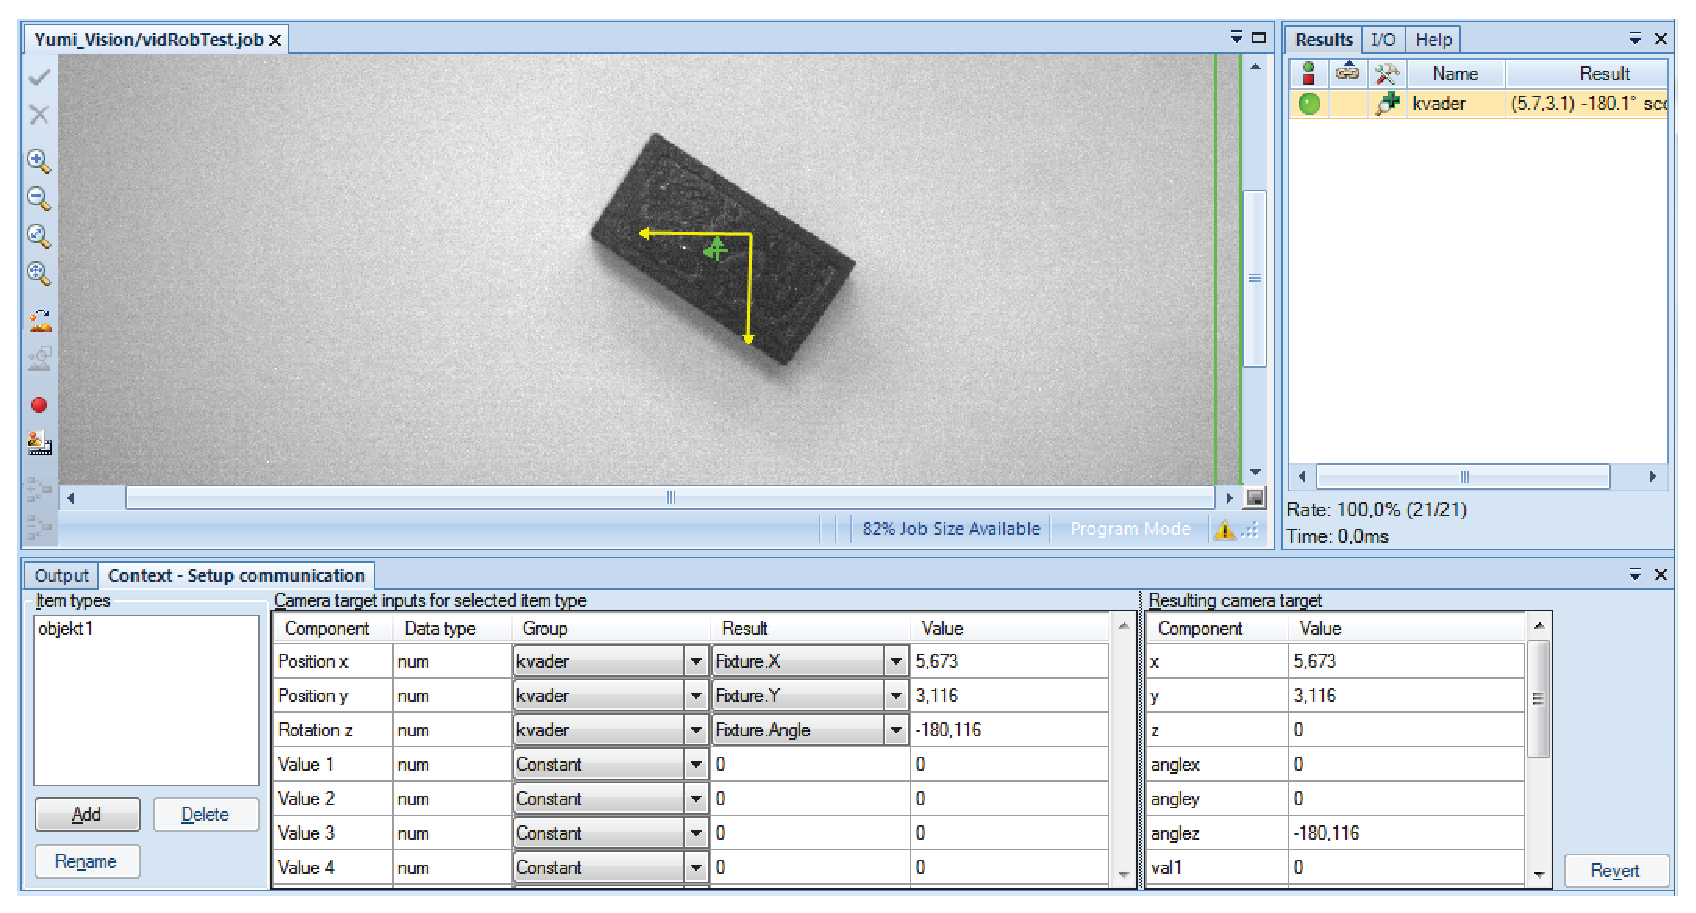
\includegraphics[width=0.9\textwidth]{yumi_rezultati2.eps}
	\caption{Primer tabele, ki povezuje podatke iz kamere s tarčno spremenljivko \emph{cameratarget}}
	\label{fig:yumi_tabela}
\end{figure}

V nadaljevanju je potrebno nastaviti povezave med orodjem za prepoznavo objektov ter robotom (RAPID programsko kodo). To se nastavi z izbiro \RS{\emph{Vision > Output to RAPID}}, ki odpre tabelo z nastavitvami (glej sliko \ref{fig:yumi_tabela}). Le-ta povezuje izhod iz orodja za prepoznavo z RAPID spremenljivko tipa \verb"cameratarget". Najprej ustrezno smiselno poimenujete objekt (\RS{\emph{Item types > Add > Rename}}). V stolpcu \RS{\emph{Group}} izberete ime orodja za prepoznavo, ki ste ga nastavili. V stolpcu \RS{\emph{Results}} definirate, katere podatke želite posredovati v RAPID kodo (pozicijo v x in y smeri, ter rotacijo okoli z osi). Na koncu shranite trenutni program.

%\begin{figure}[!hbt]
%\centering
%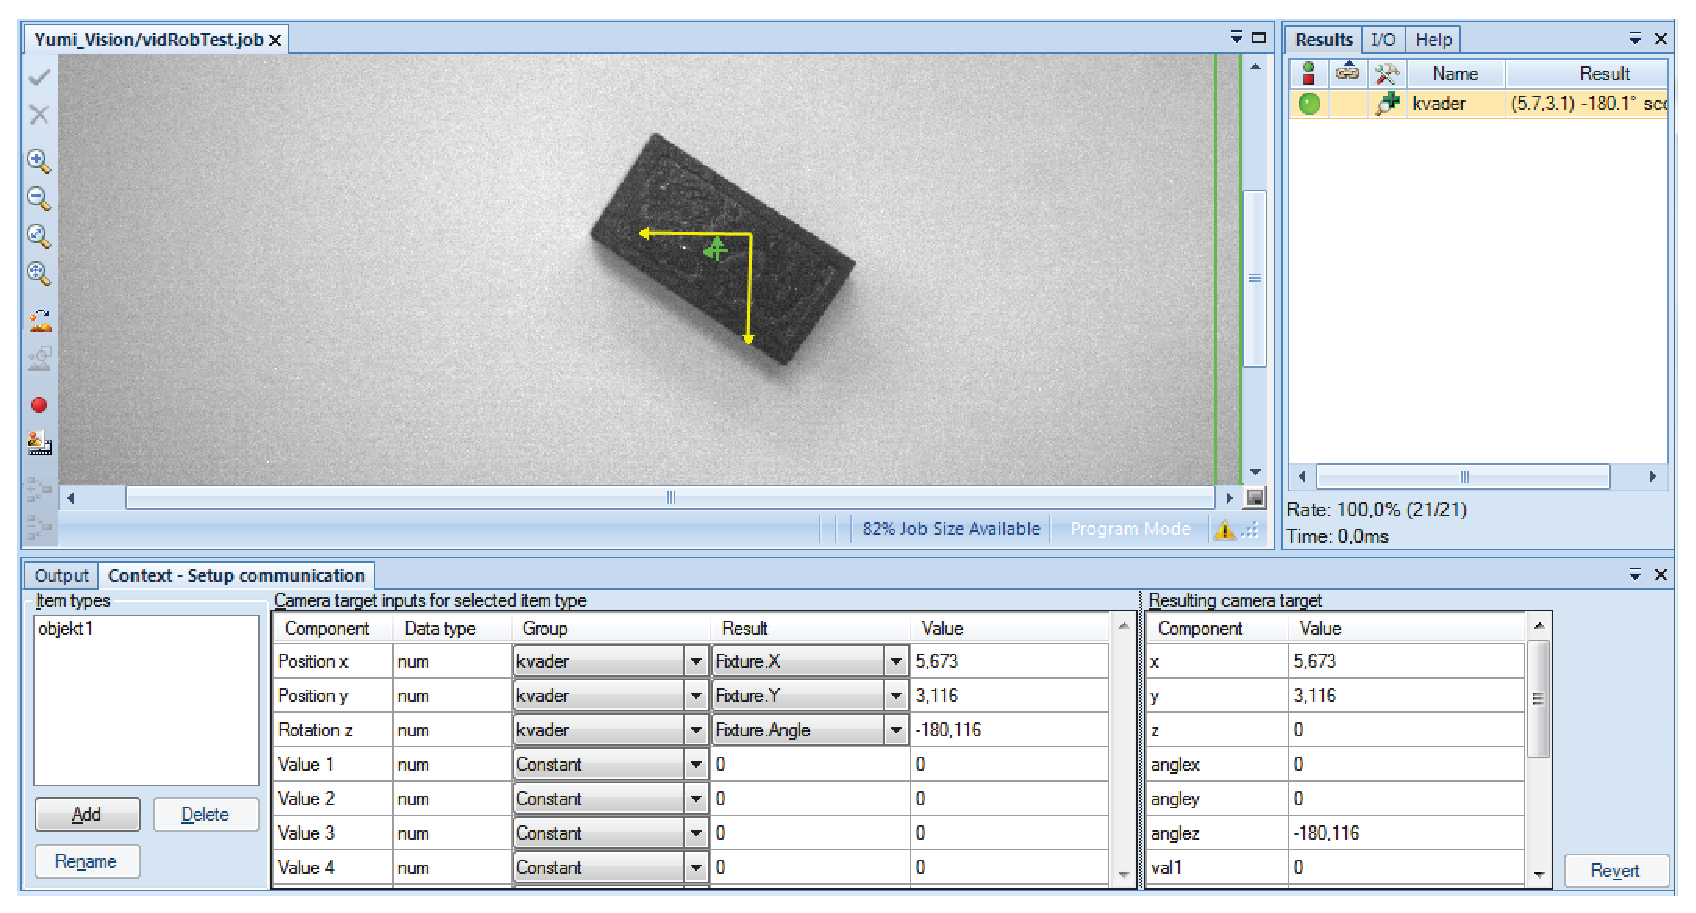
\includegraphics[width=0.9\textwidth]{yumi_rezultati2.eps}
%\caption{Primer tabele, ki povezuje podatke iz kamere s tarcno spremenljivko \emph{cameratarget}}
%\label{fig:yumi_tabela}
%\end{figure}


Ukaz v robotskem programu
%{\small
\begin{verbatim}
	CamGetResult mycamera, mycameratarget;
\end{verbatim}
%}
izvede zapis vrednosti, ki jih vrne program za prepoznavo nastavljene v \emph{Output to RAPID}, v strukturo \newline \verb"mycameratarget".


\vspace{5mm}

\begin{mdframed}[backgroundcolor=yellow!20, shadow=true,roundcorner=8pt]
	\textbf{Koraki za izvedbo naloge:}
	\begin{itemize}
		\item robota postavite v položaj za slikanje (\TP{\emph{ABB > Jogging > Go To...}}); pri tem imejte izbran delovni objekt \verb"wobj0";
		\item v vidno polje kamere postavite en objekt;
		\item zajemite sliko: \RS{\emph{Vision > Acquire Image}};
		\item nastavite ustrezne parametre slike (\RS{\emph{Vision > Setup Image}}):
		\begin{itemize}
			\item \emph{Exposure},
			\item \emph{Light Intensity};
		\end{itemize}
		\item izberite orodje za prepoznavo objektov: \RS{\emph{Vision > Add Part Location Tool > Pat Max Patterns (1-10)}}:
		\item nastavite področje modela ter področje iskanja;
		\item poimenujte orodje: \RS{\emph{Tool Name}};
		\item nastavite parametre orodja (\RS{\emph{Context - Vision tool > Settings}}):
		\begin{itemize}
			\item \emph{Number to find}: 1,
			\item \emph{Rotation Tolerance}: 90,
			\item \emph{Scale Tolerance}: 5;
		\end{itemize}
		\item testirajte delovanje orodja pri različnih postavitvah objekta;
		\item nastavite povezave med orodjem za prepoznavo ter RAPID programom: \RS{\emph{Vision > Output to RAPID}};
		\item shranite program: \RS{\emph{Vision > Save Job}}.
	\end{itemize}
\end{mdframed}


\subsection{Prijemanje in manipulacija objekta}

Pred prijemanjem morate koordinatnemu sistemu vašega delovnega objekta, ki je definiran v  \verb"mywobj" sistemu (\verb".oframe" - \emph{object frame}), prirediti vrednost (lego objekta), ki jo določite pri prepoznavi objekta s kamero (\verb".cframe" - \emph{current frame}). To stori koda
%{\small
\begin{verbatim}
	wobjKamere.oframe := mycameratarget.cframe;
\end{verbatim}
%}

Orodje, ki ga boste uporabili za pobiranje objektov, bo kar servo prijemalo, ki je nameščeno na levi robotski roki. Vrh prijemala je definiran s TCP kalibracijo z imenom \verb"GripperL", kot delovni objekt pa mora biti izbran \verb"wobjKamere". Točka prijemanja je podana z ukazom
%{\small
\begin{verbatim}
	MoveL prijemObjekta, v200, fine, GripperL
	\Wobj:=wobjKamere;
\end{verbatim}
%}

To točko je potrebno ustrezno spremeniti, da bo predstavljala lego robotskega prijemala v trenutku prijemanja. Z ročno učno napravo prezamete pravice pisanja programskemu paketu RobotStudio (izberete \TP{\emph{Revoke}}), odprete program za levo roko, postavite programski kazalec na začetek (\TP{\emph{Debug > PP to main}}) ter poženite program (fizična tipka \TP{\emph{Play}}). Program se bo izvedel do vrstice, kjer je \verb"Break". Do takrat se bo izvedla inizializacija kamere, robot se bo postavil v položaj za slikanje, kamera bo zajela sliko, program bo prepoznal objekt, njegovo pozicijo vrnil v strukturi \verb"mycameratarget", lega objekta pa se bo zapisala v delovni objekt \verb"wobjKamere". Na ročni učni enoti se bo izpisala lokacija, kje se nahaja trenutno prepoznani objekt. Preverite, če je podana lega smiselna: objekt mora biti za prepoznano število mm oddaljen od izhodišča uporabniškega koordinatnega sistema \verb"wobjKamere".

Sedaj robota ročno vodite do objekta. Pri tem pazite, da objekta ne premaknete, robota pa postavite v najbolj optimalno lego za prijemanje. Ko je robot postavljen, popravite pozicijo točke \verb"prijemObjekta" z ukazom \TP{\emph{Modify Position}}. Pri tem mora biti kot aktivni uporabniški koordinatni sistem izbran koordinatni sistem \verb"wobjKamere" (\TP{\emph{ABB > Jogging > Work Object}}).

V nadaljevanju programa dodajte še ukaz za zapiranje prijemala. S kurzorjem se postavite na ustrezno mesto v programu, ukaz pa vstavite z izbiro  \TP{\emph{Add Instruction > SmartGripper}}. Ukaz za zapiranje je \verb"Hand_GripInward" za odpiranje pa \verb"Hand_GripOutward".


Nato s programom RobotStudio ponovno prevzamete pravice pisanja ter zakomentirajte vrstico, ki vsebuje \verb"Break". To storite tako, da pred \verb"Break" postavite klicaj (\verb"!"): \verb"!Break;". Program naložite na krmilnik z \RS{\emph{RAPID > Apply}}.

Sedaj lahko program testirate. Prevzemite pravice pisanja z ročno učno napravo (\TP{\emph{Revoke}}), postavite programski kazalec na začetek (\TP{\emph{Debug > PP to main}}) ter poženite program. če je vse narejeno pravilno, se bo robot postavil na prepoznan objekt ter ga prijel.

Nato z uporabo ročnega vodenja robota definirajte še ostale potrebne točke, da robot odloži prijet objekt v ustrezno škatlo. Te točke ne smejo biti definirane v koordinatnem sistemu kamere/objekta, saj se ta spreminja glede na lego objekta. Pri tem ne pozabite uporabiti ukaz za odpiranje prijemala.


\vspace{5mm}

\begin{mdframed}[backgroundcolor=yellow!20, shadow=true,roundcorner=8pt]
	\textbf{Koraki za izvedbo naloge:}
	\begin{itemize}
		\item poženite program: \TP{\emph{Debug > PP to main}}, fizična tipka \TP{\emph{Play}};
		\item premaknite robota do objekta v položaj za prijemanje; kot delovni objekt nastavite \emph{wobjKamere};
		\item s kurzorjem se postavite na vrstico \verb"MoveL prijemObjekta ..." ter izberite \TP{\emph{Modify Position}};
		\item dodajte ukaz za zapiranje prijemala: \verb"Hand_GripInward";
		\item zakomentirajte vrstico, ki vsebuje \verb"Break";
		\item ponovno poženite program;
		\item dodajte točke/ukaze za odlaganje objekta;
		\item v vidno polje kamere postavite en objekt ter poženite program.
	\end{itemize}
\end{mdframed}


\subsection{Prepoznava in manipulacija več objektov}

Ko uspešno prepoznate, poberete in odložite en objekt, nadgradite vaš program za prepoznavo in manipulacijo več istih objektov. V nastavitvah orodja za prepoznavo \emph{Pat Max Patterns (1-10)} nastavite največje število objektov, ki jih pričakujete \RS{\emph{Context - Vision tool > Settings > Number to find}}. če program prepozna več istih objektov, se lege objektov shranijo v vektor. Ukaz \verb"CamGetResult" potem kliče en element naenkrat.


\begin{figure}[!hbt]
	\centering
	\includegraphics[width=0.9\textwidth]{yumi_OUT3.eps}
	\caption{Prepoznava več objektov: na vsak prepozna objekt se pripne koordinatni sistem, izhod v RAPID program pa so posamezni elementi vektorjev.}
	\label{fig:yumi_vision}
\end{figure}


Da poberete vse elemente, je potrebno v program vključiti ustrezno zanko. Pri tem si lahko pomagate z ukazom \verb"CamNumberOfResults", ki vrne število prepoznanih objektov, ki so še na razpolago. Primer testne kode je podan v nadaljevanju.

%\newpage

%\null

%\vspace{10mm}

%{\small
\begin{verbatim}
	VAR bool continueloop:=TRUE;
	...
	PROC main()
	...
	[del programa, ki inicializira kamero]
	...
	WHILE continueloop DO
	CamGetResult Yumi_Vision, mycameratarget;
	wobjKamere.oframe := mycameratarget.cframe;
	...
	[del programa, ki pobere/odnese/odloži objekt]
	...
	IF CamNumberOfResults(Yumi_Vision)<1 THEN
	continueloop:=FALSE;
	ENDIF
	ENDWHILE
	ENDPROC
\end{verbatim}
%}

%\newpage

%\vspace{5mm}
%\begin{tikzpicture}
%    \node [fill=green,rounded corners=5pt] {
%    \begin{minipage}{0.98\textwidth}
%        \textbf{Koraki za izvedbo naloge:}
%            \begin{itemize}
%                  \item v vidno polje kamere postavite tri enake objekte;
%%                  \item v naucenem orodju \emph{Pat Max Patterns (1-10)} popravite parameter \emph{Number to find} na 3 (zavihek \emph{Vision});
% %                 \item shranite program \emph{Vison > Save Job};
% %                 \item preverite, ce program za prepoznavo prepozna tri objekte;
% %                 \item v robotski program dodajte \verb"WHILE" zanko za pobiranje vseh objektov;
% %                 \item naložite program na krmilnik \emph{RAPID > Apply};
% %                 \item poženite program.
%          \end{itemize}
%    \end{minipage}
%    };
%\end{tikzpicture}

\vspace{5mm}

\begin{mdframed}[backgroundcolor=yellow!20, shadow=true,roundcorner=8pt]
	\textbf{Koraki za izvedbo naloge:}
	\begin{itemize}
		\item v vidno polje kamere postavite tri enake objekte;
		\item v naučenem orodju \emph{Pat Max Patterns (1-10)} popravite parameter \emph{Number to find} na 3 (zavihek \RS{\emph{Vision}});
		\item shranite program \RS{\emph{Vison > Save Job}};
		\item preverite, če program za prepoznavo prepozna tri objekte;
		\item v robotski program dodajte \verb"WHILE" zanko za pobiranje vseh objektov;
		\item naložite program na krmilnik \RS{\emph{RAPID > Apply}};
		\item poženite program.
	\end{itemize}
\end{mdframed}

\subsection{Zagon v avtomatskem načinu}

Ko preverite vaš program, da deluje v ročnem načinu (robot prepozna, pobere  in odloži tri objekte), lahko program požene v avtomatskem načinu. V tem načinu se bo robot premikal s hitrostmi, kot ste jih definirali  v programu. Najprej odprete produkcijsko okno: \TP{\emph{ABB > Production Window}}. Nato v hitrem meniju v \TP{\emph{Operator Panel}} izberete avtomatski način izvajanja (\TP{\emph{Auto}}). V meniju \TP{\emph{Task to Stop and Start}} izberete samo levo roko - T\_ROB\_L. Nato v produkcijskem oknu  kliknete \TP{\emph{PP to Main}} ter s tipko \TP{\emph{Play}} zaženete program.